\chapter{Background Research}\glsresetall
\label{cha:Research}
As a part of the implementation of a viable grasping point of objects in an environmental setting a research of state of the solutions of both object tracking and detection is necessary as well as researching full existing solutions.

\section{Object Detection and Tracking}
In order to get some understanding of the state of the art technologies used the research in split into multiple sections for different areas in the process of teaching a robot to pick groceries from a shelf.

\subsection{Object Detection}
The aim of generic object detection is to locate and classify an object in an image, sometimes including a bounding box on objects with a confidence of existence in the image. In general there are two approaches to object detection namely region proposal, which follows the traditional object detection pipeline and then classifying the each proposal into different object categories. The other approach is the regression or classification based approach by adopting a unified framework to achieve final results \citep{zhao}.
\cite{zhao} presents several solutions of both approaches and have also made a small roadmap of different popular solutions up until 2017. This is shown in \autoref{fig:deep_roadmap}.

\begin{figure}[H]
  \centering
  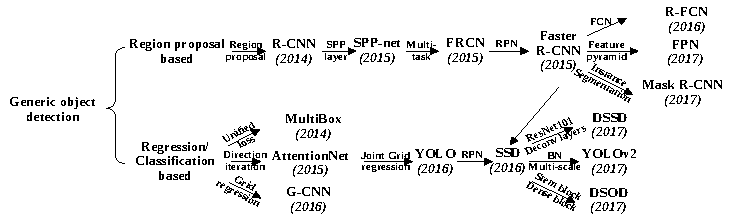
\includegraphics[width=\textwidth]{figures/deep_roadmap.pdf}
  \caption{Small roadmap of different popular solutions up until 2017 \citep{zhao}}
  \label{fig:deep_roadmap}
\end{figure}

Another way of doing object detection is using decision trees instead of deep learning as proposed by \cite{Gall2012}.

\subsubsection{Region Proposal}
The region proposal framework is a two step process. The framework firstly scans an image and then focuses in any regions in the image of interest. As shown in \autoref{fig:deep_roadmap} the R-CNN solution is one of the first in region proposal approach. The design has three stages in the process of object detection. Firstly a region proposal generation, generating 2000 region proposals for each image. Afterwards a \gls{cnn} is applied to extract features from warped or cropped regions, extracting a 4096-dimensional feature vector. From there classification and categorisation is done with pre-trained \gls{svm}s from multiple classes. The final bounding boxes are produced from adjusted scored regions using bounding box regression.

\subsubsection{Regression or Classification framework}
To compete with the time consumption of regional proposal the one-step framework based on global regression/classification is utilised by mapping straight from image pixels to bounding box coordinates and class probabilities.
This is the technique the framework \gls{yolo} applies. \gls{yolo} divides an input image into $S \times S$ grid, each cell is responsible for predicting the object centred in the cell.
The first \gls{yolo} framework has 24 convolutional layers and 2 \gls{fc} layers \citep{zhao}. The second version, referred to as both \gls{yolo}v2 and \gls{yolo}9000, uses the Darknet-19 model, which has 19 convolutional layers and 5 maxpooling layers. It is based on the Googlenet architecture \citep{Redmon2016}. At the point of deployment this framework has state of the art performance. The third iteration of the framework \gls{yolo}v3 with an update of the Darknet architecture increasing the size from 19 convolutional layers to 53. The newest \gls{yolo} framework is from early 2018 and is still one of the best in its category. In precision \cite{Redmon2018} states the framework does not perform as well as RetinaNet, but the speed of the framework is faster. \gls{yolo} is fast and lightweight enough to run in real time. It is mostly trained on the COCO and VOC datasets \citep{Redmon2018}.

\subsubsection{Decision Trees}
A decision tree consists of split nodes and leaves. The split nodes evaluate each image patch based on a set decision metric and pass the patch to either left or right in the tree. The leaf is the end of a tree and stores the statistics of the image patches which arrived during training of the tree. This is illustrated in \autoref{fig:decisiontree}.

\begin{figure}[H]
  \centering
  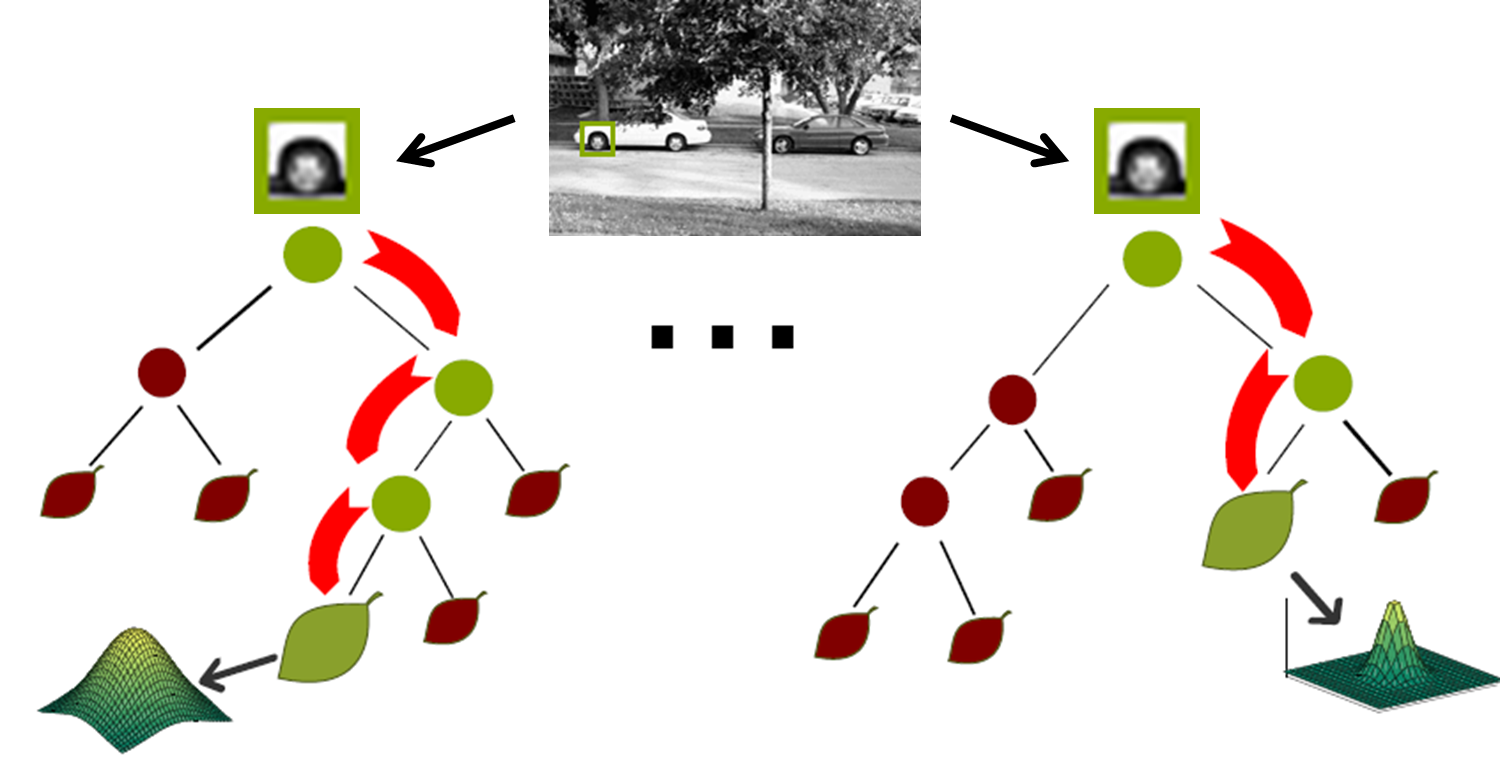
\includegraphics[width=0.7\textwidth]{figures/decisiontree}
  \caption{Example of decision tree evaluation on image patch from bounding box \citep{Gall2012}}
  \label{fig:decisiontree}
\end{figure}

\cite{Gall2012} uses a random forest for multi class object detection. A random forest consist of a set amount of decision trees.
The detection problem becomes a distribution estimation problem, where the random forests allow to learn features and descriptors that are optimal for estimating the distributions with low uncertainty. These distributions may be desirable to restrict to Gaussians or Gaussian Mixture Models \citep{Gall2012}.

The amount of training data is the most crucial parameter for detection accuracy, as random forests are designed to handle large amounts of data. If it is small training sets extra verification steps may be needed \citep{Gall2012}.

\subsection{Tracking}
General object tracking is tracking an object in a video or a sequence of images, in form of e.g. the problem of estimating the trajectory of an object in the image plane as the object moves in the image sequence. This means, that the tracker consistently labels the tracked objects in the different frames of the video \citep{Yilmaz2006}. Situations often present tracking of more than one object at the time where a multi object tracking framework is needed. \cite{Leal-Taixe2017} has evaluated on 32 different state of the art trackers from no sooner than March 2017 on multiple objects. The evaluation is performed the \gls{mot}15 and \gls{mot}16 datasets. This is done to introduce a standardised benchmark and analyse the performance of the trackers \citep{Leal-Taixe2017}. \cite{Leal-Taixe2017} states there are six top-performing trackers with a multiple object tracking accuracy higher than 40\%. 
